% #############################################################################
% This is Chapter 7
% !TEX root = ../main.tex
% #############################################################################
% Change the Name of the Chapter i the following line
\fancychapter{Results and Demonstration}
% The following line allows to ref this chapter
\label{chap:demo}

% The following line allows to ref this chapter
\label{chap:res}
This chapter presents the results of the methodology at four complementary levels: stakeholder comprehension, controlled use of generative AI, traceability-artifact automation, and the resulting stakeholder-specific Architecture Descriptions. Rather than treating generated views as the sole outcome, the chapter considers whether the methodology produces representations that stakeholders can understand, whether generative-AI output remains subject to evidence-based and human controls, and whether traceability artifacts can be created and validated consistently.

The first part of the chapter addresses viewpoint clarity and comprehension from the stakeholder perspective, followed by the controlled integration of \ac{GenAI} for validation and the partial automation of legal traceability artifacts. Together, these sections assess the practical qualities required for the methodology to be useful: comprehensibility to its intended audience, evidence grounding and human accountability, and repeatability in the handling of legal-source records.

The chapter then demonstrates the methodology through its application to \ac{DORA} and the \ac{CSA}. These applications examine how documented stakeholder responsibilities, dependencies, and concerns can be related to relevant legal requirements and materialised as stakeholder-specific \acp{AD}. For each case, the chapter presents the operational-footprint and concern analysis, regulatory-relevance and traceability results, formal viewpoint specification, and the resulting visual and textual view representations. This makes it possible to examine both the methodology's controls and automation mechanisms and its ability to produce role-relevant architectural representations of regulatory impact.
 
% #############################################################################
% #############################################################################
% #############################################################################
\section{Controlled Integration of GenAI for Validation}

\ac{GenAI} is integrated throughout the automated stages of the methodology as one layer of a controlled assurance process. It is not treated as an autonomous authority capable of proving either the factual reality of an organisation's operations or its legal compliance. Instead, the \ac{LLM} supports the extraction, structuring, comparison, and validation of evidence against the constraints defined by the methodology.

Before an artifact is materialised, the responsible agent checks that its content is grounded in approved source evidence, uses stable identifiers, and satisfies the structural rules of the relevant stage. Where information is ambiguous, incomplete, or unsupported, the process follows a zero-assumption principle: the agent must expose the uncertainty and request user input rather than infer a conclusion. This applies, for example, to operational facts and relationships, stakeholder concerns, legal relevance claims, legal-role mappings, coverage records, and view content.

The methodology combines \ac{LLM}-assisted validation with deterministic and source-based checks. 
\begin{itemize}
    \item Legal duties (\texttt{REQ-*}) are validated against the traceability matrix and the legal text;
    \item Relationship and view graphs are checked for valid endpoints, evidence, connectivity, and stakeholder presence;
    \item Generated native models(Archimate, pyArchimate or LikeC4) are checked through syntax validation, semantic validation, and, where applicable, parsing or round-trip loading.
    \item The final cross-artifact reconciliation stage verifies that the legal index, coverage ledger, viewpoint graph, textual explanation, slide diagrams, and selected native model remain mutually consistent.
\end{itemize}

User validation is therefore a required control rather than an exceptional fallback. At each approval gate, the operator may approve, reject, amend, or request further evidence for a proposed result before it is persisted. The resulting validation process provides traceability, internal consistency, evidence grounding, and technical correctness. It does not, however, replace expert legal judgement or independently establish that the organisation is compliant in practice.

\section{Partial Automation of Traceability Artifacts}

The methodology partially automates the creation and validation of traceability artifacts. Here, traceability refers to the ability to move between stakeholder interview evidence, operational facts and concerns, applicable legal duties, and the architectural representations produced later in the pipeline. Automation improves repeatability, reduces transcription errors, and makes the resulting chain of evidence easier to inspect. It does not, however, replace legal interpretation, stakeholder knowledge, or operator approval.

Once the applicable legal articles have been agreed, the agent calls the traceability matrix creator program to generate a traceability matrix. This matrix records the binding enacting terms of the selected consolidated regulation using \ac{ID}s. It acts as a human and machine readable index of the authoritative legal text, allowing the methodology to resolve a proposed legal duty to its exact legal source. The legal index is validated for its regulation and CELEX identity, expected structure, and the unique resolution of each referenced legal-text identifier.

The automation is deliberately partial. The system can generate proposed records, verify identifier resolution, detect missing anchors, check structural consistency, and preserve provenance across artifacts. It cannot independently establish that an interview statement is factually complete, that an interpretation of a legal provision is correct, or that an organisation complies with the regulation in practice. Consequently, the operator reviews and approves the legal article set, legal anchors, coverage ledger, legal-role mappings, and later reconciled artifacts before they are persisted.

\section{Architecture Description of DORA}

This section presents the application of the methodology to \ac{DORA} through three stakeholder-specific viewpoints: a Developer viewpoint, an Infrastructure and Cloud Engineer viewpoint and a Team Leader viewpoint. All viewpoints are derived from the same regulatory corpus, but represent different operational responsibilities, dependencies, concerns, and relationships with the regulation.

For each stakeholder, the methodology identifies the relevant operational footprint, maps the applicable legal requirements to the documented work context, and materialises the resulting viewpoint as an Architecture Description, while keeping user corrections only where necessary. The two cases therefore illustrate how the method can retain a common regulation-wide legal basis while producing distinct, role-relevant representations of its operational impact. The \ac{LLM} chosen for the application of the methodology was \texttt{GPT-5.6 Terra} set to Extra High reasoning, used through the Codex coding partner.

% ====================================================================================
% ====================================================================================
% ====================================================================================
% ====================================================================================
% ====================================================================================
\subsection{From the Viewpoint of a Bank Developer}

The first stakeholder to whom the methodology was applied regarding \ac{DORA} was a back-end developer of a large banking institution. This stakeholder is familiar with ArchiMate, and does have some understanding of the \ac{DORA} regulation. Below are covered the most important aspects of some of the generated artifacts, since fully listing them all would be too extensive.

\subsubsection{Operational Context and Analysis Boundary}

Through the use of a prompt containing placeholders to be replaced by the user, context and objectives were delineated.
The agent from the second step of the pipeline takes the information rich prompt the agent from the first phase helped the user make, and generates an interview, that when conducted with the stakeholder, is used to establish an operational footprint and classify the stakeholder. During these steps, the generated footprint, classification and concerns were accepted without any adjustments from the user. Assessing the interview (which can be found in the Github\footnote{\label{github}The Github for this dissertation can be found here: \url{https://github.com/AntonioBrasIST/Architecture_Viewpoints_for_EU_Regulation}}) against the resulting operational footprint, its clear the agent was capable of correctly extracting everyday tasks and dependencies, observable in \ref{tab:dora-backend-developer-profile}.

\begin{table}[ht]
\centering
\small
\begin{tabular}{p{3.2cm} p{10.2cm}}
\hline
\textbf{Dimension} & \textbf{Case profile} \\
\hline
Stakeholder and context &
Back-end Developer working on an internal Enterprise Data Platform that makes data available to other teams and services. \\
\hline
Core responsibilities &
Develops offloads, ETLs, and query services; maintains the internal framework; implements and tests code; creates pull requests; coordinates releases; and monitors production deployments. \\
\hline
Delivery path &
Works from functional specifications, performs data transformations and validation, tests in development environments, submits pull requests, opens QUA and PROD change requests, and monitors deployments through Datadog. \\
\hline
Key dependencies &
Depends on sufficiently complete specifications, read and write permissions, Team Manager and Solution Architect decisions, Infrastructure Team deployment support, and internal services such as Azure AD, Azure DevOps, Kubernetes, databases, and Kafka. \\
\hline
Decision and incident boundary &
The stakeholder implements and tests changes but does not hold final authority for architecture, functional requirements, or production approval. During incidents, the stakeholder participates in escalation and may remediate software errors owned by the responsible development team. \\
\hline
Evidence basis &
The operational footprint contains 89 approved, interview-grounded operational records, including tasks, dependencies, approvals, incident interfaces, friction points, and evidence limitations. \\
\hline
\end{tabular}
\caption{Case profile for the DORA Back-end Developer viewpoint.}
\label{tab:dora-backend-developer-profile}
\end{table}

\subsubsection{DORA Relevance and Ownership}

The extracted operational footprint and concerns are fed into the next step, the regulatory relevance analysis. This step looks trough the \ac{DORA} act searching for legal duties that will directly affect the footprint of the stakeholder, either by affecting a direct task, or by affecting the produced artifacts or some other elements that indirectly connect to the stakeholder.
The debate panel explained on section \ref{regRevAnal} unanimously retained, after structured debate, articles 7 through 13, 17, 24 and 25.
Articles 6, 14, 18 and 19 were omitted from the stakeholder scope due to there being no record of participation on the \ac{ICT} risk management framework, crisis-communication duty, incident classification duty, or competent-authority reporting responsibilities, respectively.

As a test, Article 28, requiring financial entities to manage \ac{ICT} third-party risk throughout service lifecycle, was introduced as a relevant portion of legal text that should be listed. This served as a test to check how manual interference would affect the end results and resulting regulatory relevance report, as well as introducing a requirement group that was correctly kept out of scope by the agent panel. The report successfully included all articles approved within the case scope (including 28), and listed every requirement of each article alongside the corresponding traceability matrix \ac{ID}. It is important to highlight that ownership is being taken into account when mapping requirements to the operational evidence, so that they can be reflected during view artifact generation. The distinct ownership states can be seen on table \ref{tab:dora-ownership-examples}.

\begin{table}[b]
\centering
\small
\begin{tabular}{p{2.8cm} p{10.5cm}}
\hline
\textbf{Ownership state} & \textbf{Interpretation} \\
\hline
Directly performed &
The documented maintenance work is represented as directly realizing the relevant \ac{DORA} requirement. \\
\hline
Stakeholder-constrained &
The requirement constrains the developer's work, but the developer is not presented as solely responsible for processing capacity. \\
\hline
Externally owned &
Access control is relevant to the developer's work but is represented as an externally owned dependency rather than a developer-implemented control. \\
\hline
Not evidenced / unclear owner &
The requirement affects the platform, but the interview did not establish which role or team owns its implementation. \\
\hline
\end{tabular}
\caption{Representative DORA coverage records by ownership state. The table demonstrates traceability, not organisational compliance.}
\label{tab:dora-ownership-examples}
\end{table}

Following coverage resolution, pyArchimate was selected as the technology to generate the overview View. The resulting view grouped some of the requirements \ac{DORA} mandates into 14 requirement families, observable in figure \ref{fig:dora-overview}. This provides a solid overview of the entire regulation, but not a complete, as will be observed further in \ref{chap:infra-DORA-rel-owner}.
\begin{figure}[htbp]
  \centering
  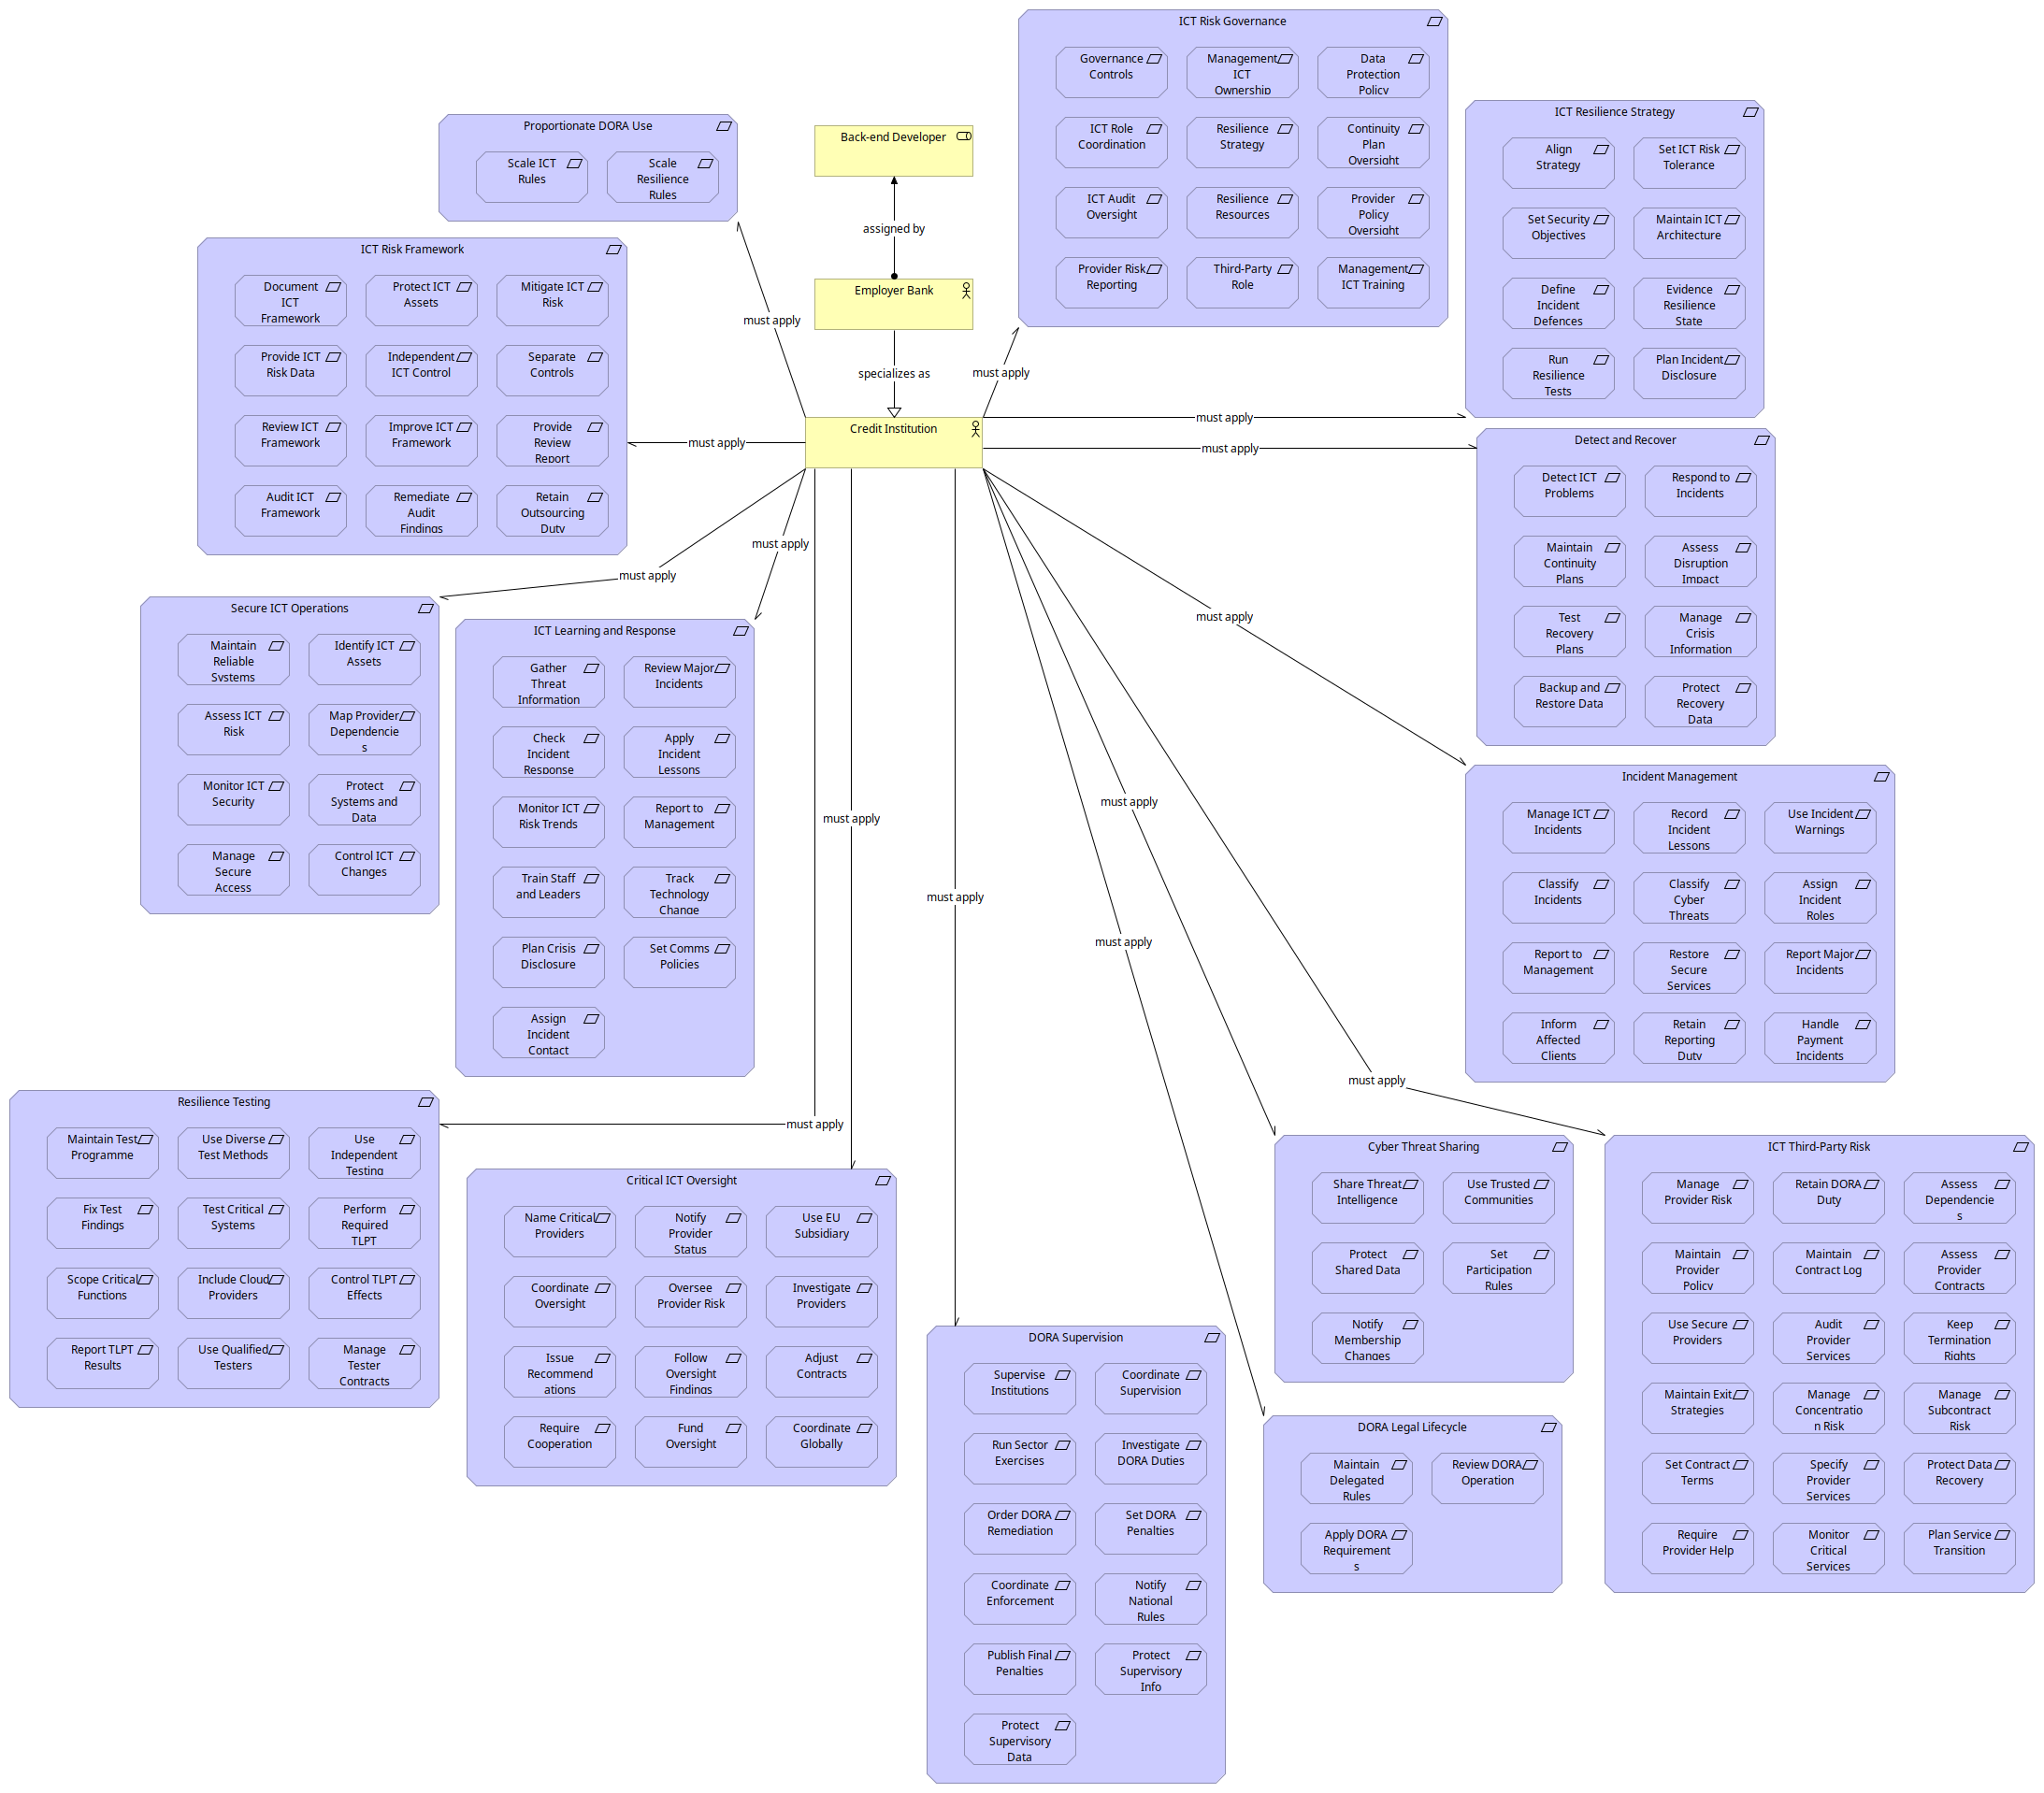
\includegraphics[width=1\textwidth]{Images/DORAOverview.png} 
  \caption{\ac{DORA} requirements overview}
  \label{fig:dora-overview}
\end{figure}

The viewpoint scope was limited to the developer's evidenced platform work and the \ac{DORA} duties that affect it. The resulting boundary includes framework maintenance, platform development, data offload work, testing and developer readiness, controlled releases, production monitoring, incident interfaces, and the user added Microsoft-cloud dependency. Everything else was excluded from direct stakeholder responsibility where the interview did not support such an attribution. These matters remain represented either as external dependencies, unclear ownership boundaries, or contextual information.

The scope was then materialised into a formal ArchiMate viewpoint. Rather than producing a single large diagram, the viewpoint separates the stakeholder-relevant regulatory impact into six connected thematic views: \ac{ICT} Asset Governance, Protection and Change, Detection and Continuity, Incident Learning, Resilience Testing, and Microsoft Cloud Risk. A separate regulation overview view preserves the wider \ac{DORA} legal context. This overview does not represent daily work or make a compliance claim. Its purpose is to establish the legal context in which the stakeholder-specific views are interpreted.

The viewpoint has a designing purpose: It makes approved \ac{DORA} constraints, ownership states, and operational relationships usable in the resulting \ac{AD} without asserting enterprise compliance. Its primary concerns are:
\begin{itemize}
    \item Cloud service provider contract risk;
    \item Change, testing, and incident interfaces;
    \item Platform, monitoring, continuity, recovery, and remediation constraints.
\end{itemize}
 These concerns are formalised into six connected thematic views, using nested requirement families and evidence-backed ArchiMate relationships.


\subsubsection{Resulting Architecture Description}

The approved viewpoint was materialised as a pyArchimate \ac{AD}, preserving the approved operational evidence, legal requirements, ownership states, and ArchiMate relationships.

The resulting \ac{AD} contains a regulation overview view and six stakeholder-specific thematic views: \ac{ICT} Asset Governance, Protection and Change, Detection and Continuity, Incident Learning, Resilience Testing, and Microsoft Cloud Risk.

The Resilience Testing view, shown in Figure \ref{fig:dora-resilience-testing}, represents testing and developer readiness activities, pull-request creation, and the separate Technical Reviewer role. It demonstrates that testing duties directly connected to the developer are represented differently from review activities whose ownership was not established by the interview evidence. It also shows the requirements that constrain the developer, as well as the realized requirements. Every view can be observed in the Github\footref{github}.

\begin{figure}[htbp]
  \centering
  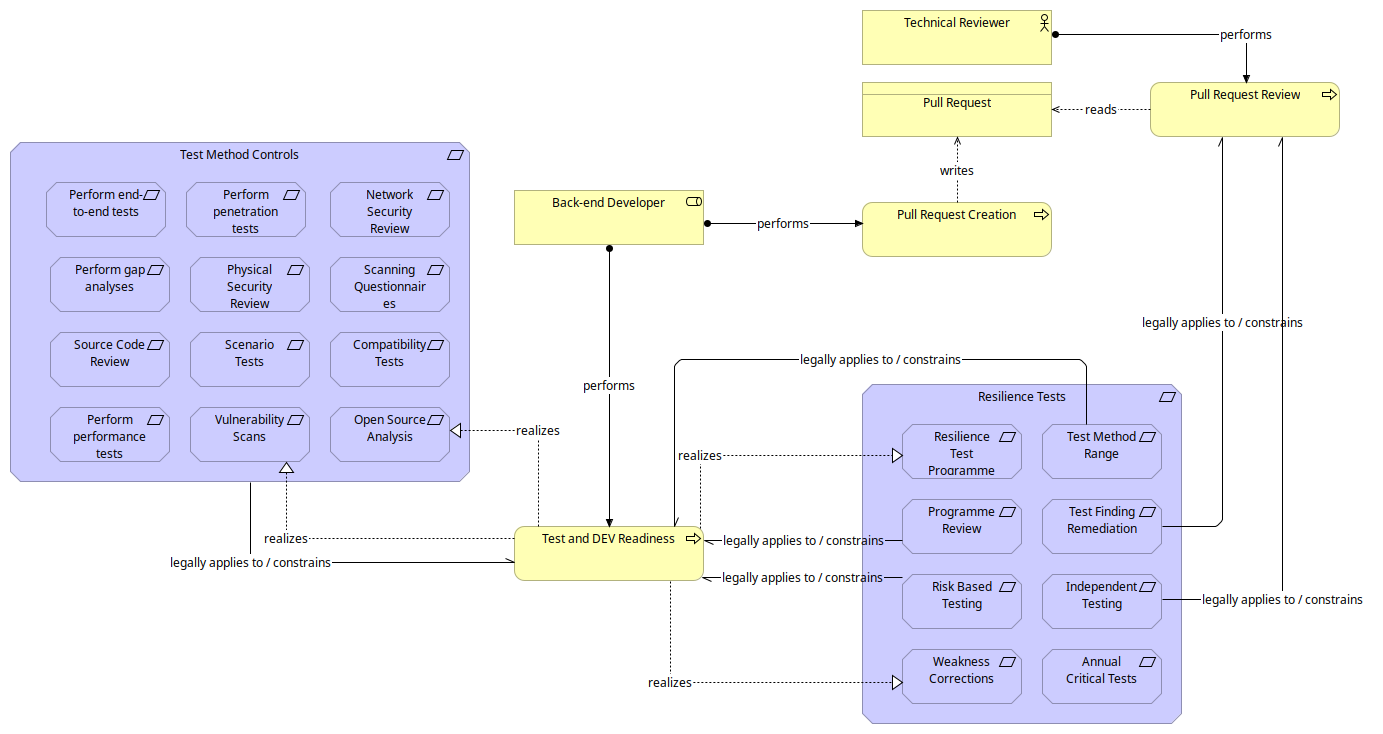
\includegraphics[width=1\textwidth]{Images/dora-resilience-testing.png} 
  \caption{\ac{DORA} Bank Developer Resilience Testing View}
  \label{fig:dora-resilience-testing}
\end{figure}

It is also of interest to look at the generated view for Microsoft Cloud Risk, depicted in \ref{fig:dev-microsoft-cloud-risk}. While the view may look weak at a first glance, it is important to note that operational queues given by the stakeholder during the interview make no mention of a contract with Microsoft, only implications. Additionally, these concerns do not affect the footprint of the stakeholder in any way. The view should not exist in the first place, and would not exist had it not been force-included by the user during the requirement elicitation phase. Therefore, the view was generated in accordance with existing operational evidence and did not make assumptions. The developer is not affected by these requirements, only the entity employing the developer is. 

\begin{figure}[b]
  \centering
  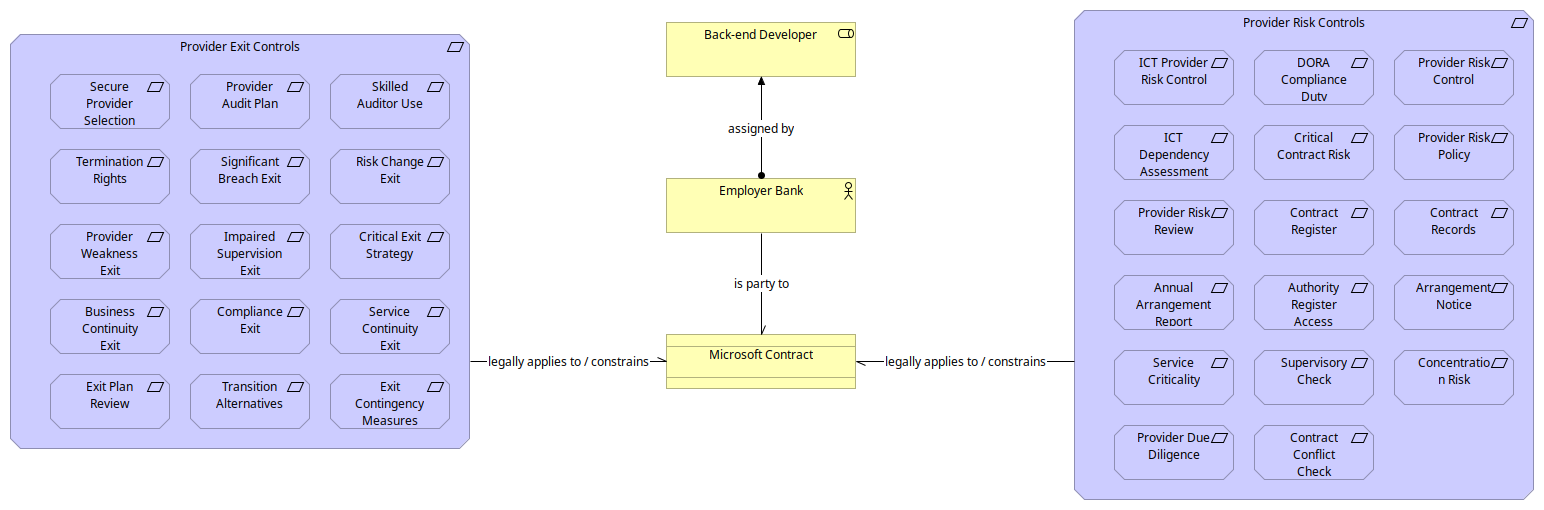
\includegraphics[width=1\textwidth]{Images/Dev_Microsoft_Cloud_Risk.png} 
  \caption{\ac{DORA} Bank Developer Microsoft Cloud Risk View}
  \label{fig:dev-microsoft-cloud-risk}
\end{figure}

A textual explanation and condensed Markdown slide diagrams complement the formal views by explaining their operational meaning and presenting their main relationships in a more accessible format. However, these initiatives have either underperformed against their objectives or demand additional development to reach their complete value. These short-comings are further addressed in \ref{chap:infra-res-AD}

Still, the case demonstrates that the methodology can translate \ac{DORA} into a stakeholder-specific \ac{AD} while preserving the distinction between direct technical work, external organisational controls, and areas in which the interview evidence does not establish ownership.

% ====================================================================================
\subsection{From the Viewpoint of a Bank Infrastructure and Cloud Engineer}

The second stakeholder was a Infrastructure and Cloud engineer of a banking institution, carrying database administrator responsibilities. This stakeholder had no detailed knowledge of \ac{DORA} and was unfamiliar with Archimate.

Regardless, the overall feedback provided by the stakeholder was positive. In fact, the stakeholder gained a new understanding of some requirements enforced by \ac{DORA}, and what processes were affected by them.

The following sub-sections review some sections of the artifacts produced by the methodology in greater detail. 

\subsubsection{Operational Context and Analysis Boundary}

The process began with an optimized prompt oriented towards interview building. The agent deemed it had enough information, so placeholders were not necessary.
Next, an interview was generated, and sent to the stakeholder. Due to having been sent and not conducted, feedback from the stakeholder indicated the sensation that the questions were too vague. Regardless, the answers given received were rich on information and processes subject to \ac{DORA}. The footprint and concerns derived from these answers were considered to be accurate by the stakeholder, and can be found in \ref{tab:dora-infra-cloud-dba-profile}.

\begin{table}[ht]
\centering
\small
\begin{tabular}{p{3.2cm} p{10.2cm}}
\hline
\textbf{Dimension} & \textbf{Case profile} \\
\hline
Stakeholder and context &
Infrastructure Engineer / Cloud Database Administrator working in the internal data technology layer of a \ac{DORA}-regulated financial entity. The stakeholder administers Starburst, OpenMetadata, and SingleStore. \\
\hline
Core responsibilities &
Provisions user access, investigates developer connection and technology-usage issues, maintains technologies through updates and configuration changes, partly automates access-control work, validates changes, and supports incident response. \\
\hline
Delivery path &
Maintains YAML configurations through Git and VS Code; performs changes such as Starburst GitOps migration and Flux-based configuration deployment to \ac{AKS}; tests updates in non-production environments; and validates changes through logs, service checks, and database-connection queries. Production changes are recorded in ServiceNow and proceed only after stability testing and the absence of reported user issues. \\
\hline
Key dependencies &
Depends on the \ac{AKS}/compute team for underlying infrastructure support, the networking team for connection issues, technology support teams for specialised correction, the security team for access-request approval, and the authorisation team for production-change approval. Key operational systems include Ranger, Flux, Azure DevOps, Azure Key Vault, Datadog, and an internal ticketing system. \\
\hline
Decision and incident boundary &
The stakeholder's team is accountable for the technologies it configures, but the stakeholder may not alter information without an approved DevOps change. Production-change authorisation and access approval are performed by dedicated teams. During SingleStore outages, the stakeholder restarts, investigates, and mitigates the service, while escalating to the team lead, other DevOps leads, or technology support as required, and produces a post-incident report. \\
\hline
Evidence basis &
The operational footprint contains 58 approved operational records. These comprise user-approved role context and interview-grounded tasks, technology responsibilities, dependencies, approval constraints, incident interfaces, friction points, and explicitly recorded evidence gaps. \\
\hline
\end{tabular}
\caption{Case profile for the \ac{DORA} Infrastructure  and  Cloud Engineer viewpoint.}
\label{tab:dora-infra-cloud-dba-profile}
\end{table}

\subsubsection{DORA Relevance and Ownership}
\label{chap:infra-DORA-rel-owner}

Regulatory relevance against \ac{DORA} promptly followed the stakeholder classification. The panel outputted articles 6 through 14, 17, 18, 24 and 25. Omissions and exclusions where:
\begin{itemize}
    \item \textbf{Article 5 — Governance and organisation:} Was omitted due to the panel never agreeing on it. This is correct, since the \ac{ICT} risk control framework mentioned in it is directed to the management body, whom this stakeholder is not a part of.
    \item \textbf{Article 19 — Reporting of major ICT-related incidents and voluntary notification of significant cyber threats:} Excluded unanimously after debate. Also a correct decision, due to communication to competent authorities not falling within the operational footprint of the stakeholder.
    \item \textbf{Article 28 — General principles:} Also excluded unanimously after debate. This article establishes entity-level management of \ac{ICT} third-party risk, meaning that excluding it from the relevant list of relevant requirements was also a correct decision.
\end{itemize}
The requirements outlined in the selected articles were considered accurate selections and included in the resulting relevance regulatory report.

After relevance resolution, pyArchimate was selected as the technology to generate the overview View. Unlike the view for the developer, instead of having separate requirement families, every requirement family was nested within a \ac{DORA} Resilience Framework requirement, as can be observed in figure \ref{fig:dora-overview-infra}.

\begin{figure}[htbp]
  \centering
  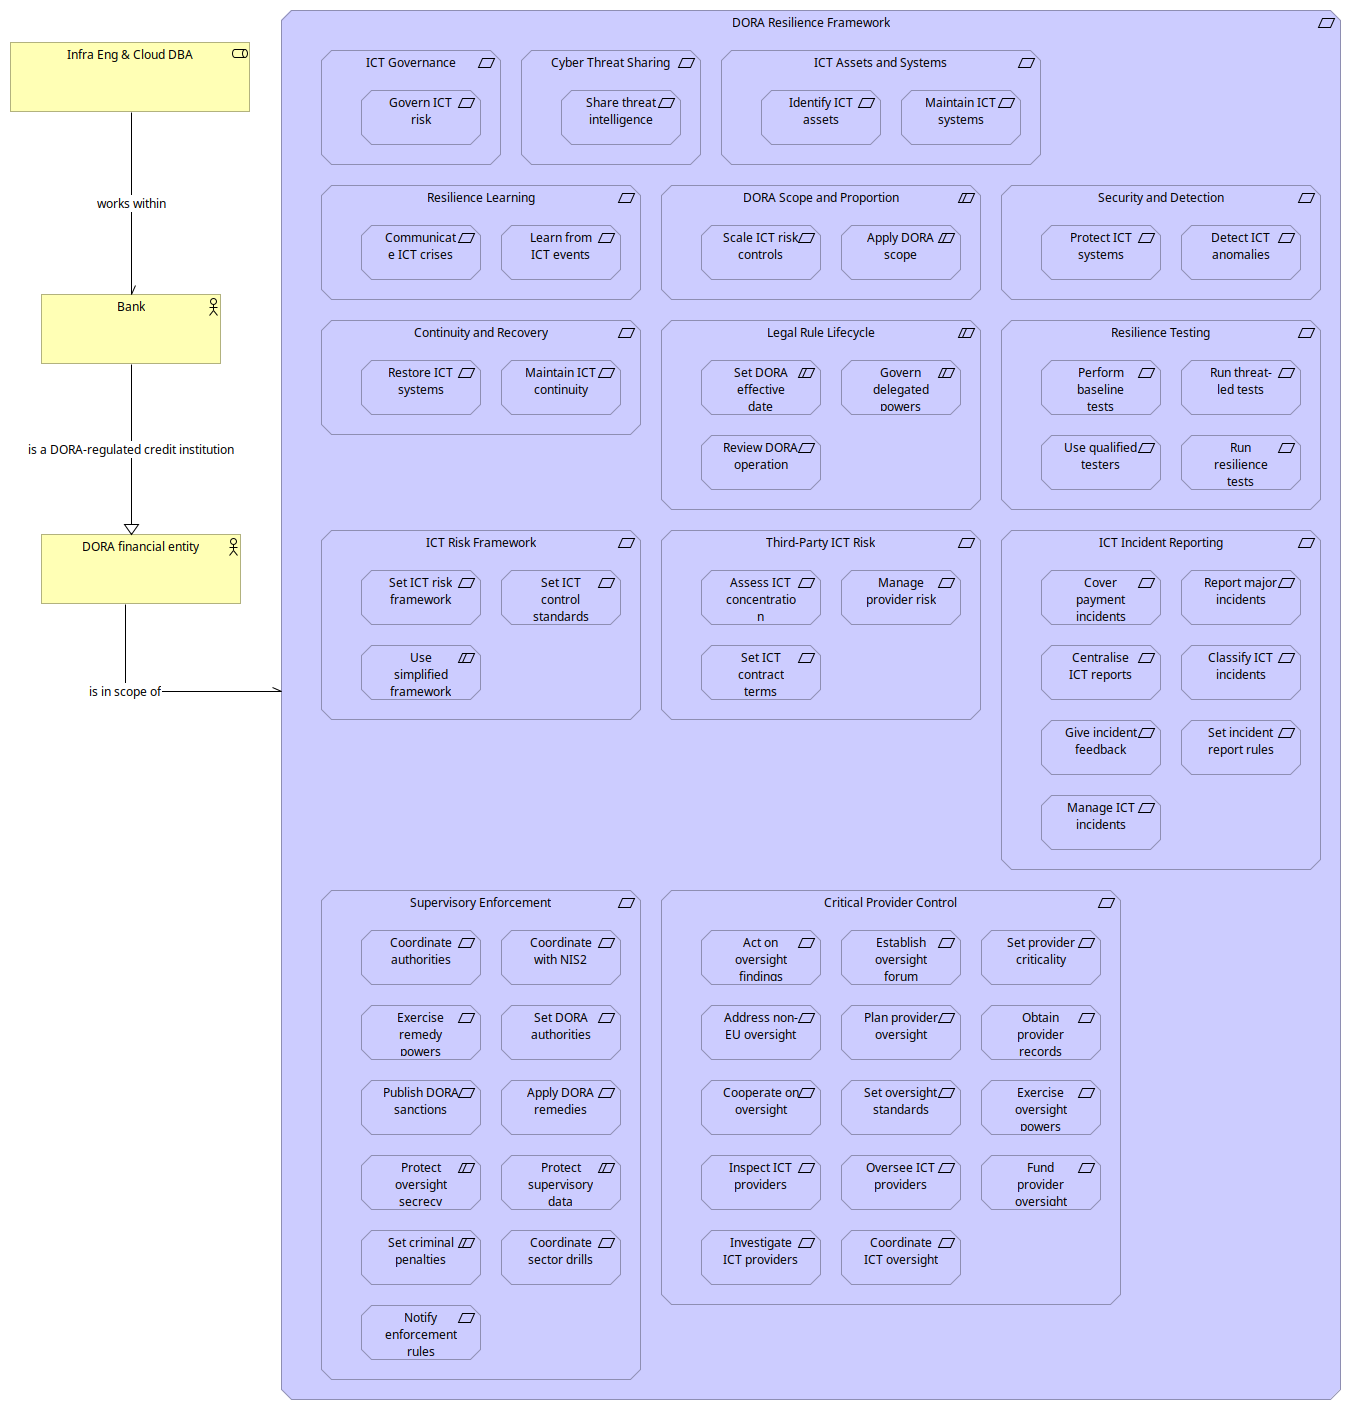
\includegraphics[width=1\textwidth]{Images/DORARegulationOverview_infra.png} 
  \caption{\ac{DORA} Infra and Cloud Engineer Requirements Overview}
  \label{fig:dora-overview-infra}
\end{figure}

The grouping of the requirement families within the overall \ac{DORA} Resilience Framework requirement is the first detail, when comparing with the previous overview view \ref{fig:dora-overview}, that comes to attention.

Another difference is that while \ref{fig:dora-overview} has 134 requirements, \ref{fig:dora-overview-infra} has only 57. However, this is a better result. The back-end developer overview view has a lot of depth, which is not intended for an overview view. These 134 requirements cover only 44 legal articles out of a 64 total. \ref{fig:dora-overview-infra} covers 57 distinct articles, meaning each requirement is derived from an article. Since the overview is intended to be a high-level depiction of the whole regulation meant for stakeholder awareness, this is the better result amongst the two.

Both observations are attributed to the non-deterministic nature of \ac{LLM}s, since nothing was done differently in order to achieve distinct results.

Viewpoint scoping then organised all coverage relationships from the relevance report into fourteen legal requirement families and a role-specific operational-context stream. The scope focused on the stakeholder's administration of Starburst, OpenMetadata, and SingleStore, encompassing access control, configuration, controlled change, monitoring, incident response, recovery, and testing. Enterprise-wide governance, authority reporting, audit ownership, and other responsibilities not evidenced as belonging to the stakeholder remained outside the direct stakeholder boundary.

The resulting viewpoint, named \textit{DORA Infrastructure Resilience}, was defined for the Infrastructure and Cloud Engineer. Its purpose is informing: it presents the relationship between the stakeholder's approved operational context and the relevant \ac{DORA} requirements without assessing organisational compliance. The viewpoint addresses governance, administrative, and technical concerns through requirement families covering, among other topics, platform management, access and security, monitoring, continuity, recovery, incident handling, and resilience testing.

\subsubsection{Resulting Architecture Description}
\label{chap:infra-res-AD}

The viewpoint materialisation produced seventeen connected views: the immutable \ac{DORA} overview, thirteen legal thematic views, and three operational-context views. The latter could not be connected to any specific \ac{DORA} requirements, hence being modelled only as operational-context views.
The thirteen legal thematic views are:
\begin{itemize}
    \item ICT Risk Governance
    \item Platform \& Asset Management
    \item Provider Dependencies
    \item Access \& Security
    \item Controlled Change
    \item Monitoring \& Detection
    \item Continuity Preparedness
    \item Recovery \& Restoration
    \item Operational Learning
    \item Crisis Communication
    \item Incident Management
    \item Incident Classification
    \item Resilience Testing 
\end{itemize}

The Controlled Change view, observable in figure \ref{fig:controlled-change-view} represents the approval change path for a production-change. The view was deemed accurate by the stakeholder, with possible improvements, providing preliminary stakeholder-based evidence that the second objective of the work was achieved. These observations are discussed in \ref{observations}.

The generated textual explanation provided a per-view walk-through of every element and relation paired with an ``Why it appears'' explanation. The condensed Markdown slide diagrams identified presented a simplified version of every view. 

\begin{figure}[t]
  \centering
  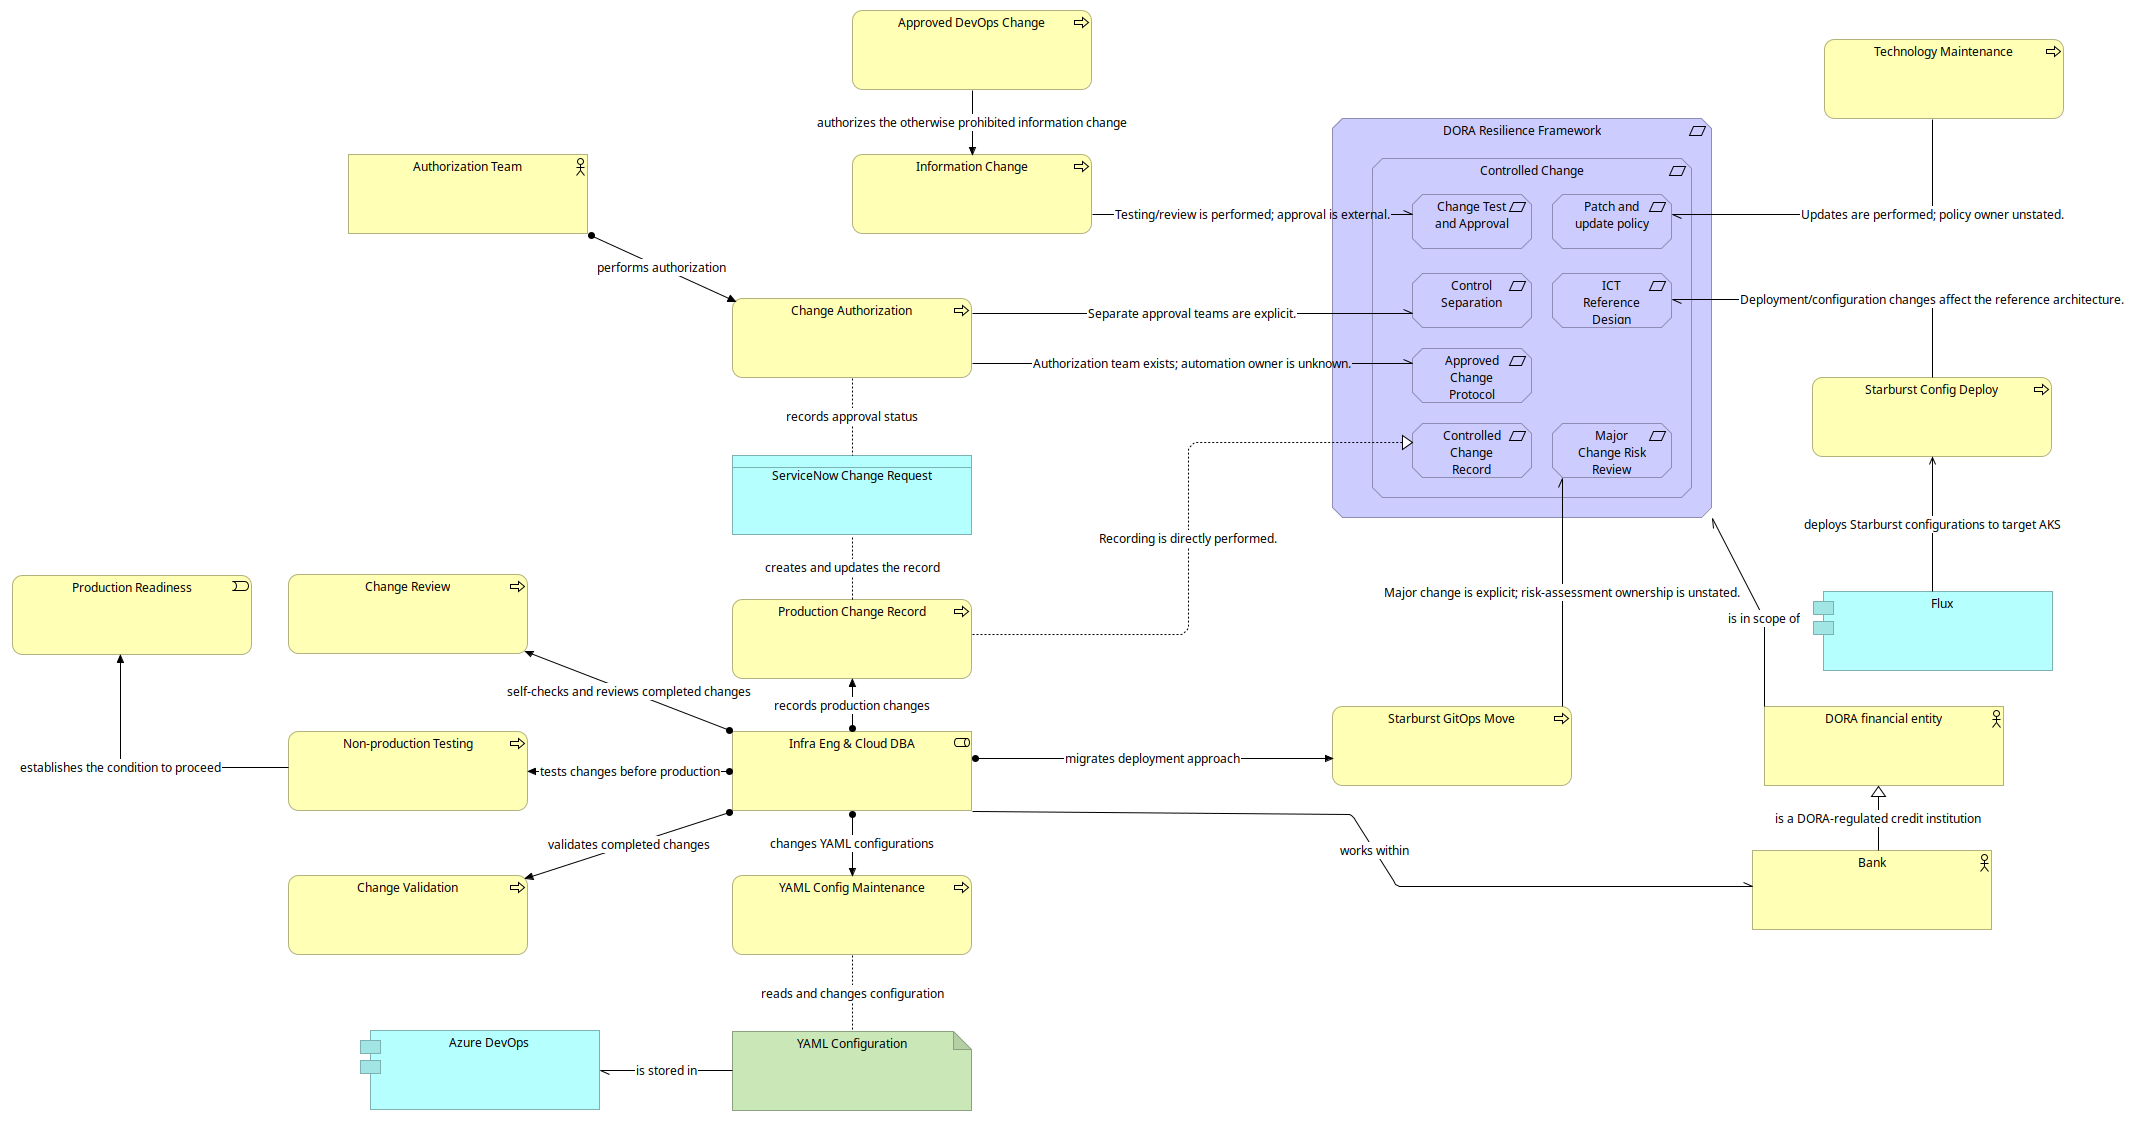
\includegraphics[width=1\textwidth]{Images/Controlled Change.png} 
  \caption{\ac{DORA} Infra and Cloud Engineer ''Controlled Change`` View}
  \label{fig:controlled-change-view}
\end{figure}

% ====================================================================================
%\subsection{From the Viewpoint of a Bank Team Leader}

%\texttt{ADICIONAR OPINIÃO DESTE STAKEHOLDER SOBRE AS VISTAS}
%\subsection{From a Compliance Officer's Viewpoint}

%\texttt{ADICIONAR OPINIÃO DESTE STAKEHOLDER SOBRE AS VISTAS}



% #############################################################################
% #############################################################################
\section{Observations from the Demonstration}
\label{observations}

During the showing of the generated views and explanatory artifacts to their respective stakeholders , observations were made by the stakeholders regarding the \ac{AD}s and registered. These form a strong basis of what is working as intended in the method, and what could be improved in the future. Regarding the views, they are as follows: 
% feedback Gonçalo
\begin{itemize}
    \item Realization relations should be used when a requirement is realized by processes not directly performed by the stakeholder. Only using the realization relations for tasks realized directly by the stakeholder was found to be confusing.
    \item One major change directly realized by the stakeholder was not connected to a requirement regarding risk reviews for major changes. Upon footprint re-assessment, the risk review was left unmentioned by the stakeholder during the interview, meaning that the relation was correctly attributed as an association, and that it should be replaced with a realization.
    \item The stakeholder also mentioned that some elements were too abstract. What was represented in the view was correct and made sense, however what should be represented was an abstraction of the specific business process itself. (i.e., instead of ``Starburst GitOps Move'' should have been ``Major technology move'').
    %\item Text in some of the relations was confusing.
\end{itemize}

Regarding the textual explanation, feedback expressed that it could be a useful idea, but the current texts need improvement. This is because the \ac{LLM} currently explains \textit{what} and \textit{why} in the context of the methodology, and not in the operational context of the stakeholder. Examples of this can be found in every stakeholder textual explanation artifact. From the Infrastructure engineer textual explanation artifact, the provided explanation for the ``Reliable \ac{ICT} systems'' requirement is ``Atomic DORA requirement: Reliable ICT systems. It represents COV-002 under ICT Asset Controls (Art. 7)''. Although correct, the \textit{what} does not justify what the requirement is in detail, and the \textit{why} omits to explain what in the operational context is affected by the requirement. Improvements can be made on this subject so that the explanation provides the operational narrative needed by the stakeholder.

Feedback about the markdown slides was received poorly in the collected feedback. Although they were intended to provide an accessible summary of the formal views, their simplification frequently removed contextual detail and relationships necessary to convey the intended regulatory and operational message. As a result, they introduced a substantial loss of semantic clarity rather than improving comprehension.

Moreover, participants with no prior knowledge of ArchiMate were able to interpret the formal diagrams with relative ease when supported by the descriptions and traceability matrix. This suggests that the simplified slides do not provide sufficient additional value to justify their reduced fidelity. Future iterations of the methodology should therefore discontinue the use of these simplified slide artefacts and instead prioritise the formal ArchiMate views, complemented where necessary by stakeholder-oriented textual explanations.

%\texttt{Falta adicionar o que o Team Lead disser depois da demo}